\documentclass[10pt,a4paper,openright]{article}
\usepackage{amsfonts}
\usepackage{float}
\usepackage[utf8]{inputenc}
\usepackage[T1]{fontenc}
\usepackage{graphicx}
\usepackage{amsmath,amssymb,verbatim}
\textheight=240mm
\textwidth=170mm
\topmargin=-15mm
\oddsidemargin=-6mm
\evensidemargin=\oddsidemargin
\newcommand\tab[1][1cm]{\hspace*{#1}}
\usepackage{hyperref}
\newcommand{\norm}[1]{\left\lVert#1\right\rVert}

\begin{document}
	\begin{flushleft}
		\large Name: Matouš Dzivjak\\
		\large Date: 3.11.2018\\
	\end{flushleft}
\begin{center}
	\huge Identifikace autoregresního modelu
\end{center}
\section{Zadání}
\begin{verbatim}
https://gitlab.fel.cvut.cz/B0B33OPT/public/blob/master/cviceni/02_ar_model/02_ar_model.pdf
\end{verbatim}


\section{Řešení}
\subsection{}
\begin{center}
Z rovnice 2 v zadání dostaneme matici $M$ a vektor $b$
\end{center}

\[M=
\begin{bmatrix}
1 & y_{p-1} & \dots & y_{0} \\
1 & y_{p} & \dots & y_{1}  \\
1 & y_{p+1} & \dots & y_{2}\\
\vdots & \vdots & \vdots &\vdots \\
1 & y_{T-1} & \dots & y_{T-p}
\end{bmatrix}\]

\[b=
\begin{bmatrix}
y_{p} \\
 y_{p+1}  \\
 y_{p+2}\\
\vdots \\
 y_{T}
\end{bmatrix}\]

\subsection{}
\begin{center}
Implementace algoritmu řešící problém nejmenších čtverců pomocí QR rozkladu je v kódu.
$\norm{\hat{a}_{1} - \hat{a}_{2}} = 6.1739 \cdot 10^{-13}$ \\
kde $\hat{a}_{1}$ je výsledek funkce $A\textbackslash b$ a $\hat{a}_{2}$ je výsledek funkce $solve\_ls\left(A,b\right)$
\end{center}

\subsection{}
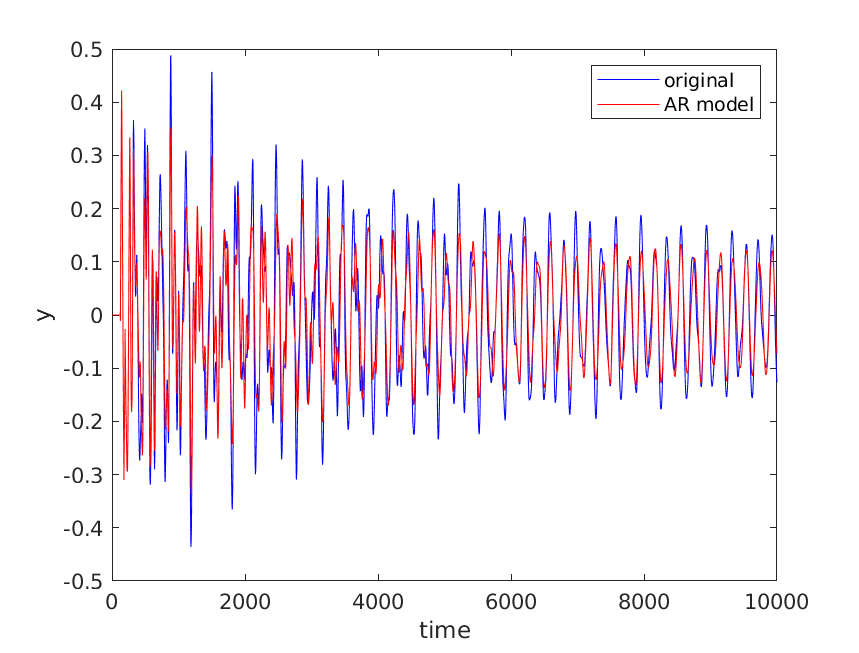
\includegraphics[scale=0.8]{graph.png}
\end{document}